\documentclass[1p]{elsarticle_modified}
%\bibliographystyle{elsarticle-num}

%\usepackage[colorlinks]{hyperref}
%\usepackage{abbrmath_seonhwa} %\Abb, \Ascr, \Acal ,\Abf, \Afrak
\usepackage{amsfonts}
\usepackage{amssymb}
\usepackage{amsmath}
\usepackage{amsthm}
\usepackage{scalefnt}
\usepackage{amsbsy}
\usepackage{kotex}
\usepackage{caption}
\usepackage{subfig}
\usepackage{color}
\usepackage{graphicx}
\usepackage{xcolor} %% white, black, red, green, blue, cyan, magenta, yellow
\usepackage{float}
\usepackage{setspace}
\usepackage{hyperref}

\usepackage{tikz}
\usetikzlibrary{arrows}

\usepackage{multirow}
\usepackage{array} % fixed length table
\usepackage{hhline}

%%%%%%%%%%%%%%%%%%%%%
\makeatletter
\renewcommand*\env@matrix[1][\arraystretch]{%
	\edef\arraystretch{#1}%
	\hskip -\arraycolsep
	\let\@ifnextchar\new@ifnextchar
	\array{*\c@MaxMatrixCols c}}
\makeatother %https://tex.stackexchange.com/questions/14071/how-can-i-increase-the-line-spacing-in-a-matrix
%%%%%%%%%%%%%%%

\usepackage[normalem]{ulem}

\newcommand{\msout}[1]{\ifmmode\text{\sout{\ensuremath{#1}}}\else\sout{#1}\fi}
%SOURCE: \msout is \stkout macro in https://tex.stackexchange.com/questions/20609/strikeout-in-math-mode

\newcommand{\cancel}[1]{
	\ifmmode
	{\color{red}\msout{#1}}
	\else
	{\color{red}\sout{#1}}
	\fi
}

\newcommand{\add}[1]{
	{\color{blue}\uwave{#1}}
}

\newcommand{\replace}[2]{
	\ifmmode
	{\color{red}\msout{#1}}{\color{blue}\uwave{#2}}
	\else
	{\color{red}\sout{#1}}{\color{blue}\uwave{#2}}
	\fi
}

\newcommand{\Sol}{\mathcal{S}} %segment
\newcommand{\D}{D} %diagram
\newcommand{\A}{\mathcal{A}} %arc


%%%%%%%%%%%%%%%%%%%%%%%%%%%%%5 test

\def\sl{\operatorname{\textup{SL}}(2,\Cbb)}
\def\psl{\operatorname{\textup{PSL}}(2,\Cbb)}
\def\quan{\mkern 1mu \triangleright \mkern 1mu}

\theoremstyle{definition}
\newtheorem{thm}{Theorem}[section]
\newtheorem{prop}[thm]{Proposition}
\newtheorem{lem}[thm]{Lemma}
\newtheorem{ques}[thm]{Question}
\newtheorem{cor}[thm]{Corollary}
\newtheorem{defn}[thm]{Definition}
\newtheorem{exam}[thm]{Example}
\newtheorem{rmk}[thm]{Remark}
\newtheorem{alg}[thm]{Algorithm}

\newcommand{\I}{\sqrt{-1}}
\begin{document}

%\begin{frontmatter}
%
%\title{Boundary parabolic representations of knots up to 8 crossings}
%
%%% Group authors per affiliation:
%\author{Yunhi Cho} 
%\address{Department of Mathematics, University of Seoul, Seoul, Korea}
%\ead{yhcho@uos.ac.kr}
%
%
%\author{Seonhwa Kim} %\fnref{s_kim}}
%\address{Center for Geometry and Physics, Institute for Basic Science, Pohang, 37673, Korea}
%\ead{ryeona17@ibs.re.kr}
%
%\author{Hyuk Kim}
%\address{Department of Mathematical Sciences, Seoul National University, Seoul 08826, Korea}
%\ead{hyukkim@snu.ac.kr}
%
%\author{Seokbeom Yoon}
%\address{Department of Mathematical Sciences, Seoul National University, Seoul, 08826,  Korea}
%\ead{sbyoon15@snu.ac.kr}
%
%\begin{abstract}
%We find all boundary parabolic representation of knots up to 8 crossings.
%
%\end{abstract}
%\begin{keyword}
%    \MSC[2010] 57M25 
%\end{keyword}
%
%\end{frontmatter}

%\linenumbers
%\tableofcontents
%
\newcommand\colored[1]{\textcolor{white}{\rule[-0.35ex]{0.8em}{1.4ex}}\kern-0.8em\color{red} #1}%
%\newcommand\colored[1]{\textcolor{white}{ #1}\kern-2.17ex	\textcolor{white}{ #1}\kern-1.81ex	\textcolor{white}{ #1}\kern-2.15ex\color{red}#1	}

{\Large $\underline{12a_{0295}~(K12a_{0295})}$}

\setlength{\tabcolsep}{10pt}
\renewcommand{\arraystretch}{1.6}
\vspace{1cm}\begin{tabular}{m{100pt}>{\centering\arraybackslash}m{274pt}}
\multirow{5}{120pt}{
	\centering
	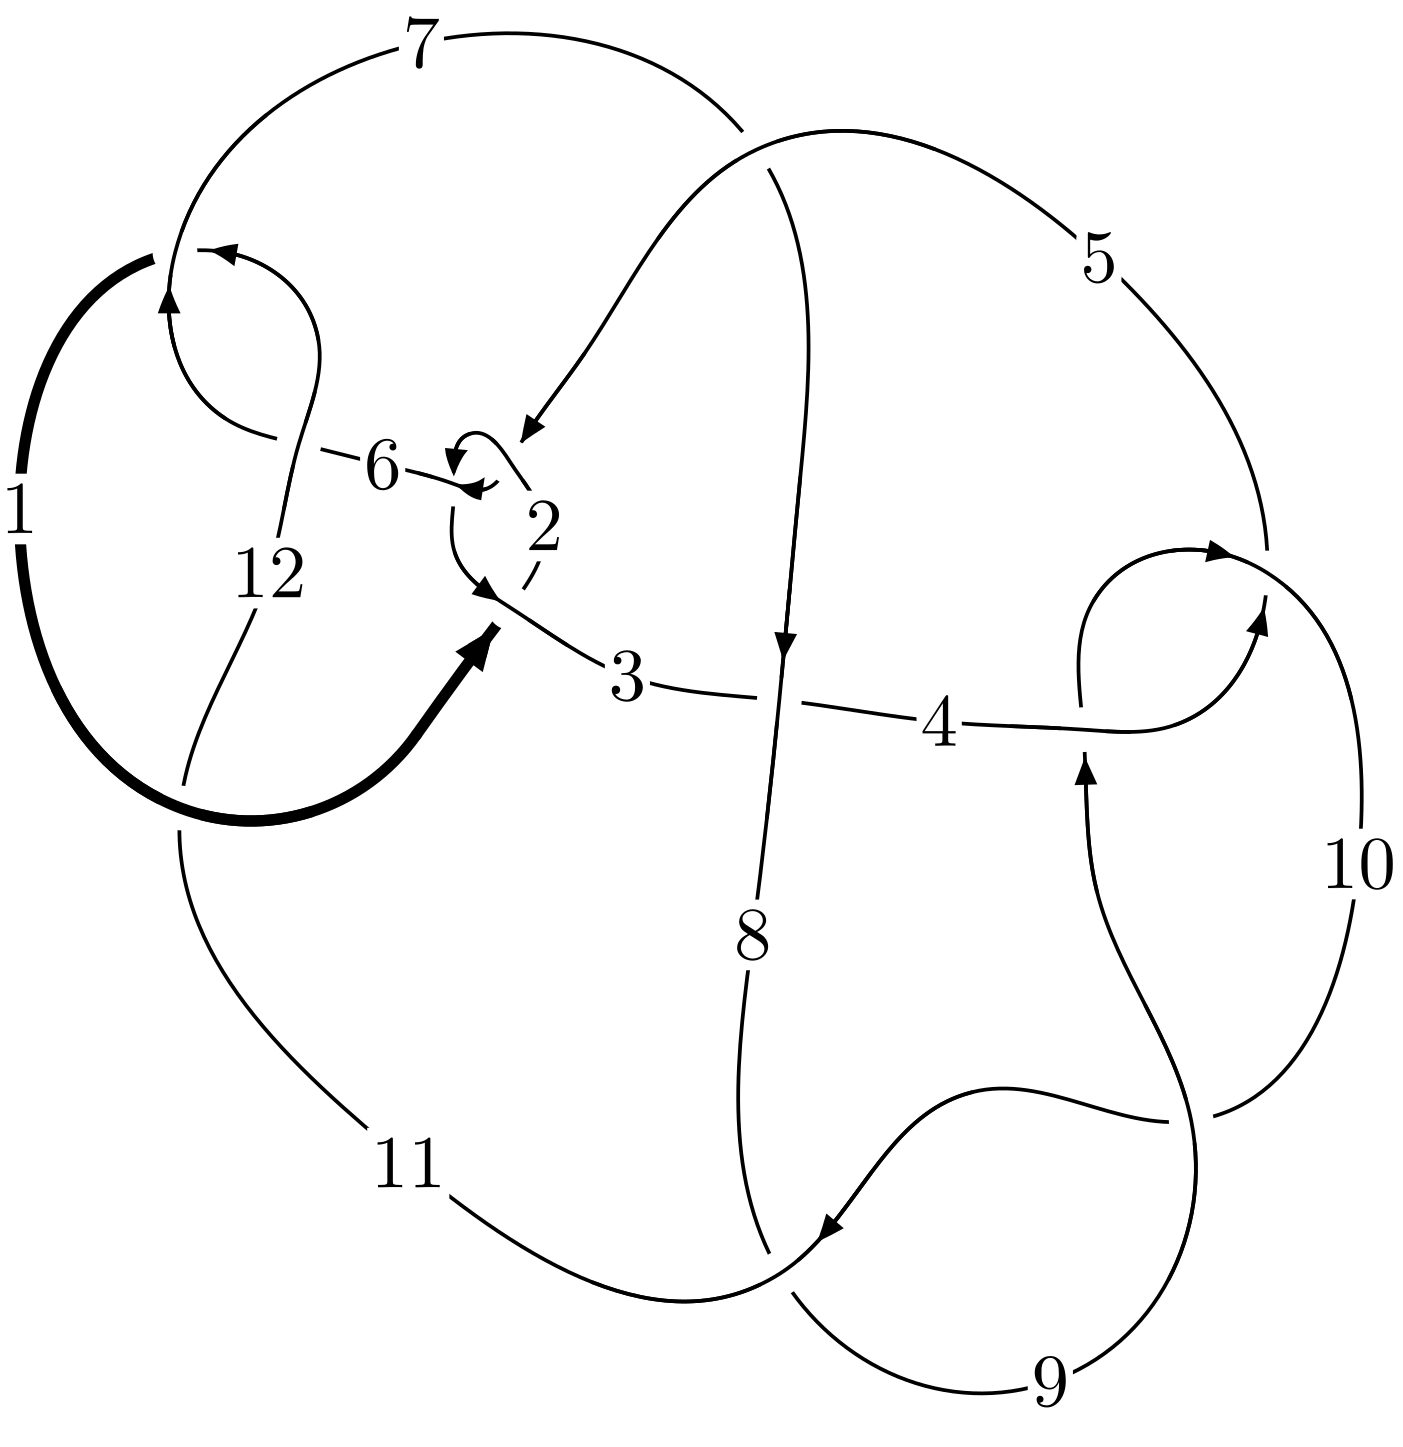
\includegraphics[width=112pt]{../../../GIT/diagram.site/Diagrams/png/1096_12a_0295.png}\\
\ \ \ A knot diagram\footnotemark}&
\allowdisplaybreaks
\textbf{Linearized knot diagam} \\
\cline{2-2}
 &
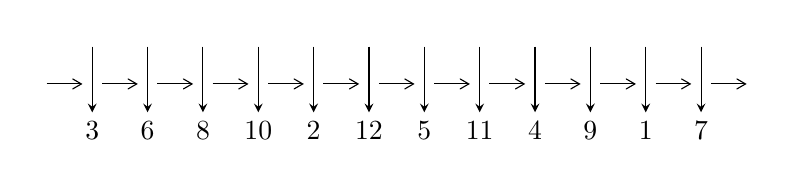
\begin{tikzpicture}[x=20pt, y=17pt]
	% nodes
	\node (C0) at (0, 0) {};
	\node (C1) at (1, 0) {};
	\node (C1U) at (1, +1) {};
	\node (C1D) at (1, -1) {3};

	\node (C2) at (2, 0) {};
	\node (C2U) at (2, +1) {};
	\node (C2D) at (2, -1) {6};

	\node (C3) at (3, 0) {};
	\node (C3U) at (3, +1) {};
	\node (C3D) at (3, -1) {8};

	\node (C4) at (4, 0) {};
	\node (C4U) at (4, +1) {};
	\node (C4D) at (4, -1) {10};

	\node (C5) at (5, 0) {};
	\node (C5U) at (5, +1) {};
	\node (C5D) at (5, -1) {2};

	\node (C6) at (6, 0) {};
	\node (C6U) at (6, +1) {};
	\node (C6D) at (6, -1) {12};

	\node (C7) at (7, 0) {};
	\node (C7U) at (7, +1) {};
	\node (C7D) at (7, -1) {5};

	\node (C8) at (8, 0) {};
	\node (C8U) at (8, +1) {};
	\node (C8D) at (8, -1) {11};

	\node (C9) at (9, 0) {};
	\node (C9U) at (9, +1) {};
	\node (C9D) at (9, -1) {4};

	\node (C10) at (10, 0) {};
	\node (C10U) at (10, +1) {};
	\node (C10D) at (10, -1) {9};

	\node (C11) at (11, 0) {};
	\node (C11U) at (11, +1) {};
	\node (C11D) at (11, -1) {1};

	\node (C12) at (12, 0) {};
	\node (C12U) at (12, +1) {};
	\node (C12D) at (12, -1) {7};
	\node (C13) at (13, 0) {};

	% arrows
	\draw[->,>={angle 60}]
	(C0) edge (C1) (C1) edge (C2) (C2) edge (C3) (C3) edge (C4) (C4) edge (C5) (C5) edge (C6) (C6) edge (C7) (C7) edge (C8) (C8) edge (C9) (C9) edge (C10) (C10) edge (C11) (C11) edge (C12) (C12) edge (C13) ;	\draw[->,>=stealth]
	(C1U) edge (C1D) (C2U) edge (C2D) (C3U) edge (C3D) (C4U) edge (C4D) (C5U) edge (C5D) (C6U) edge (C6D) (C7U) edge (C7D) (C8U) edge (C8D) (C9U) edge (C9D) (C10U) edge (C10D) (C11U) edge (C11D) (C12U) edge (C12D) ;
	\end{tikzpicture} \\
\hhline{~~} \\& 
\textbf{Solving Sequence} \\ \cline{2-2} 
 &
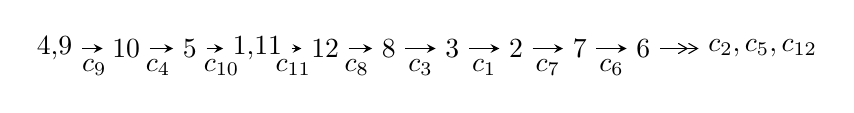
\begin{tikzpicture}[x=23pt, y=7pt]
	% node
	\node (A0) at (-1/8, 0) {4,9};
	\node (A1) at (1, 0) {10};
	\node (A2) at (2, 0) {5};
	\node (A3) at (49/16, 0) {1,11};
	\node (A4) at (33/8, 0) {12};
	\node (A5) at (41/8, 0) {8};
	\node (A6) at (49/8, 0) {3};
	\node (A7) at (57/8, 0) {2};
	\node (A8) at (65/8, 0) {7};
	\node (A9) at (73/8, 0) {6};
	\node (C1) at (1/2, -1) {$c_{9}$};
	\node (C2) at (3/2, -1) {$c_{4}$};
	\node (C3) at (5/2, -1) {$c_{10}$};
	\node (C4) at (29/8, -1) {$c_{11}$};
	\node (C5) at (37/8, -1) {$c_{8}$};
	\node (C6) at (45/8, -1) {$c_{3}$};
	\node (C7) at (53/8, -1) {$c_{1}$};
	\node (C8) at (61/8, -1) {$c_{7}$};
	\node (C9) at (69/8, -1) {$c_{6}$};
	\node (A10) at (11, 0) {$c_{2},c_{5},c_{12}$};

	% edge
	\draw[->,>=stealth]	
	(A0) edge (A1) (A1) edge (A2) (A2) edge (A3) (A3) edge (A4) (A4) edge (A5) (A5) edge (A6) (A6) edge (A7) (A7) edge (A8) (A8) edge (A9) ;
	\draw[->>,>={angle 60}]	
	(A9) edge (A10);
\end{tikzpicture} \\ 

\end{tabular} \\

\footnotetext{
The image of knot diagram is generated by the software ``\textbf{Draw programme}" developed by Andrew Bartholomew(\url{http://www.layer8.co.uk/maths/draw/index.htm\#Running-draw}), where we modified some parts for our purpose(\url{https://github.com/CATsTAILs/LinksPainter}).
}\phantom \\ \newline 
\centering \textbf{Ideals for irreducible components\footnotemark of $X_{\text{par}}$} 
 
\begin{align*}
I^u_{1}&=\langle 
3 u^{45}-6 u^{44}+\cdots+b+3,\;-7 u^{45}+17 u^{44}+\cdots+2 a-14,\;u^{46}-3 u^{45}+\cdots+4 u-2\rangle \\
I^u_{2}&=\langle 
33684 u^{32} a-254577 u^{32}+\cdots+7807 a-17533,\;2 u^{32} a-5 u^{32}+\cdots-4 a+3,\;u^{33}+2 u^{32}+\cdots-2 u-1\rangle \\
I^u_{3}&=\langle 
- u^2+b- u+1,\;u^3+2 a+u-2,\;u^4- u^2+2\rangle \\
I^u_{4}&=\langle 
b-1,\;a+1,\;u+1\rangle \\
I^u_{5}&=\langle 
b+1,\;a+1,\;u-1\rangle \\
I^u_{6}&=\langle 
b,\;a+1,\;u-1\rangle \\
I^u_{7}&=\langle 
b-1,\;a,\;u-1\rangle \\
I^u_{8}&=\langle 
- u^3- u^2+b-1,\;u^3+u^2+a- u,\;u^4+1\rangle \\
\\
I^v_{1}&=\langle 
a,\;b-1,\;v+1\rangle \\
\end{align*}
\raggedright * 9 irreducible components of $\dim_{\mathbb{C}}=0$, with total 125 representations.\\
\footnotetext{All coefficients of polynomials are rational numbers. But the coefficients are sometimes approximated in decimal forms when there is not enough margin.}
\newpage
\renewcommand{\arraystretch}{1}
\centering \section*{I. $I^u_{1}= \langle 3 u^{45}-6 u^{44}+\cdots+b+3,\;-7 u^{45}+17 u^{44}+\cdots+2 a-14,\;u^{46}-3 u^{45}+\cdots+4 u-2 \rangle$}
\flushleft \textbf{(i) Arc colorings}\\
\begin{tabular}{m{7pt} m{180pt} m{7pt} m{180pt} }
\flushright $a_{4}=$&$\begin{pmatrix}0\\u\end{pmatrix}$ \\
\flushright $a_{9}=$&$\begin{pmatrix}1\\0\end{pmatrix}$ \\
\flushright $a_{10}=$&$\begin{pmatrix}1\\u^2\end{pmatrix}$ \\
\flushright $a_{5}=$&$\begin{pmatrix}- u\\- u^3+u\end{pmatrix}$ \\
\flushright $a_{1}=$&$\begin{pmatrix}\frac{7}{2} u^{45}-\frac{17}{2} u^{44}+\cdots-10 u+7\\-3 u^{45}+6 u^{44}+\cdots+7 u-3\end{pmatrix}$ \\
\flushright $a_{11}=$&$\begin{pmatrix}- u^2+1\\u^2\end{pmatrix}$ \\
\flushright $a_{12}=$&$\begin{pmatrix}-\frac{3}{2} u^{45}+\frac{7}{2} u^{44}+\cdots+4 u-2\\u^{45}-2 u^{44}+\cdots-3 u+1\end{pmatrix}$ \\
\flushright $a_{8}=$&$\begin{pmatrix}u^4- u^2+1\\- u^4\end{pmatrix}$ \\
\flushright $a_{3}=$&$\begin{pmatrix}u^9-2 u^7+3 u^5-2 u^3+u\\- u^9+u^7- u^5+u\end{pmatrix}$ \\
\flushright $a_{2}=$&$\begin{pmatrix}\frac{3}{2} u^{45}-\frac{7}{2} u^{44}+\cdots-5 u+3\\- u^{45}+2 u^{44}+\cdots+2 u-1\end{pmatrix}$ \\
\flushright $a_{7}=$&$\begin{pmatrix}- u^8+u^6- u^4+1\\- u^{10}+2 u^8-3 u^6+2 u^4- u^2\end{pmatrix}$ \\
\flushright $a_{6}=$&$\begin{pmatrix}\frac{3}{2} u^{45}-\frac{3}{2} u^{44}+\cdots-3 u-1\\2 u^{45}-7 u^{44}+\cdots-7 u+7\end{pmatrix}$\\&\end{tabular}
\flushleft \textbf{(ii) Obstruction class $= -1$}\\~\\
\flushleft \textbf{(iii) Cusp Shapes $= -2 u^{45}-8 u^{44}+\cdots-2 u+4$}\\~\\
\newpage\renewcommand{\arraystretch}{1}
\flushleft \textbf{(iv) u-Polynomials at the component}\newline \\
\begin{tabular}{m{50pt}|m{274pt}}
Crossings & \hspace{64pt}u-Polynomials at each crossing \\
\hline $$\begin{aligned}c_{1},c_{11}\end{aligned}$$&$\begin{aligned}
&u^{46}+19 u^{45}+\cdots+19 u+1
\end{aligned}$\\
\hline $$\begin{aligned}c_{2},c_{5},c_{6}\\c_{12}\end{aligned}$$&$\begin{aligned}
&u^{46}+u^{45}+\cdots-3 u-1
\end{aligned}$\\
\hline $$\begin{aligned}c_{3}\end{aligned}$$&$\begin{aligned}
&u^{46}+3 u^{45}+\cdots-1200 u-194
\end{aligned}$\\
\hline $$\begin{aligned}c_{4},c_{9}\end{aligned}$$&$\begin{aligned}
&u^{46}-3 u^{45}+\cdots+4 u-2
\end{aligned}$\\
\hline $$\begin{aligned}c_{7}\end{aligned}$$&$\begin{aligned}
&u^{46}-21 u^{45}+\cdots-27796 u+2962
\end{aligned}$\\
\hline $$\begin{aligned}c_{8},c_{10}\end{aligned}$$&$\begin{aligned}
&u^{46}+15 u^{45}+\cdots+24 u+4
\end{aligned}$\\
\hline
\end{tabular}\\~\\
\newpage\renewcommand{\arraystretch}{1}
\flushleft \textbf{(v) Riley Polynomials at the component}\newline \\
\begin{tabular}{m{50pt}|m{274pt}}
Crossings & \hspace{64pt}Riley Polynomials at each crossing \\
\hline $$\begin{aligned}c_{1},c_{11}\end{aligned}$$&$\begin{aligned}
&y^{46}+29 y^{45}+\cdots-83 y+1
\end{aligned}$\\
\hline $$\begin{aligned}c_{2},c_{5},c_{6}\\c_{12}\end{aligned}$$&$\begin{aligned}
&y^{46}-19 y^{45}+\cdots-19 y+1
\end{aligned}$\\
\hline $$\begin{aligned}c_{3}\end{aligned}$$&$\begin{aligned}
&y^{46}-3 y^{45}+\cdots-95192 y+37636
\end{aligned}$\\
\hline $$\begin{aligned}c_{4},c_{9}\end{aligned}$$&$\begin{aligned}
&y^{46}-15 y^{45}+\cdots-24 y+4
\end{aligned}$\\
\hline $$\begin{aligned}c_{7}\end{aligned}$$&$\begin{aligned}
&y^{46}+9 y^{45}+\cdots-47342296 y+8773444
\end{aligned}$\\
\hline $$\begin{aligned}c_{8},c_{10}\end{aligned}$$&$\begin{aligned}
&y^{46}+33 y^{45}+\cdots-448 y+16
\end{aligned}$\\
\hline
\end{tabular}\\~\\
\newpage\flushleft \textbf{(vi) Complex Volumes and Cusp Shapes}
$$\begin{array}{c|c|c}  
\text{Solutions to }I^u_{1}& \I (\text{vol} + \sqrt{-1}CS) & \text{Cusp shape}\\
 \hline 
\begin{aligned}
u &= -0.987506 + 0.181737 I \\
a &= \phantom{-}0.353118 - 0.157922 I \\
b &= \phantom{-}1.104500 + 0.248593 I\end{aligned}
 & -0.01578 + 1.44584 I & -12.13380 - 1.16212 I \\ \hline\begin{aligned}
u &= -0.987506 - 0.181737 I \\
a &= \phantom{-}0.353118 + 0.157922 I \\
b &= \phantom{-}1.104500 - 0.248593 I\end{aligned}
 & -0.01578 - 1.44584 I & -12.13380 + 1.16212 I \\ \hline\begin{aligned}
u &= \phantom{-}0.624787 + 0.751761 I \\
a &= \phantom{-}0.501815 - 1.195750 I \\
b &= \phantom{-}0.27921 + 1.52890 I\end{aligned}
 & -1.03505 - 2.62041 I & -12.25047 + 5.62134 I \\ \hline\begin{aligned}
u &= \phantom{-}0.624787 - 0.751761 I \\
a &= \phantom{-}0.501815 + 1.195750 I \\
b &= \phantom{-}0.27921 - 1.52890 I\end{aligned}
 & -1.03505 + 2.62041 I & -12.25047 - 5.62134 I \\ \hline\begin{aligned}
u &= \phantom{-}0.932010 + 0.249601 I \\
a &= -0.114325 - 0.813437 I \\
b &= -0.108703 + 0.755311 I\end{aligned}
 & \phantom{-}0.48280 - 3.89081 I & -12.3138 + 7.4640 I \\ \hline\begin{aligned}
u &= \phantom{-}0.932010 - 0.249601 I \\
a &= -0.114325 + 0.813437 I \\
b &= -0.108703 - 0.755311 I\end{aligned}
 & \phantom{-}0.48280 + 3.89081 I & -12.3138 - 7.4640 I \\ \hline\begin{aligned}
u &= \phantom{-}1.03795\phantom{ +0.000000I} \\
a &= -0.425099\phantom{ +0.000000I} \\
b &= \phantom{-}0.441184\phantom{ +0.000000I}\end{aligned}
 & -5.06706\phantom{ +0.000000I} & -16.3430\phantom{ +0.000000I} \\ \hline\begin{aligned}
u &= -0.656480 + 0.675086 I \\
a &= \phantom{-}0.421198 + 0.564603 I \\
b &= \phantom{-}0.364479 - 0.548670 I\end{aligned}
 & -0.056532 - 0.529762 I & -9.92309 + 2.36241 I \\ \hline\begin{aligned}
u &= -0.656480 - 0.675086 I \\
a &= \phantom{-}0.421198 - 0.564603 I \\
b &= \phantom{-}0.364479 + 0.548670 I\end{aligned}
 & -0.056532 + 0.529762 I & -9.92309 - 2.36241 I \\ \hline\begin{aligned}
u &= \phantom{-}0.957126 + 0.460438 I \\
a &= -0.173508 + 1.059270 I \\
b &= \phantom{-}0.660431 - 0.373019 I\end{aligned}
 & -2.47921 + 5.69529 I & -15.9789 - 3.1429 I\\
 \hline 
 \end{array}$$\newpage$$\begin{array}{c|c|c}  
\text{Solutions to }I^u_{1}& \I (\text{vol} + \sqrt{-1}CS) & \text{Cusp shape}\\
 \hline 
\begin{aligned}
u &= \phantom{-}0.957126 - 0.460438 I \\
a &= -0.173508 - 1.059270 I \\
b &= \phantom{-}0.660431 + 0.373019 I\end{aligned}
 & -2.47921 - 5.69529 I & -15.9789 + 3.1429 I \\ \hline\begin{aligned}
u &= -1.069760 + 0.055455 I \\
a &= -0.606557 - 0.782831 I \\
b &= \phantom{-}0.110005 - 0.642276 I\end{aligned}
 & -6.77795 - 3.22325 I & -19.8771 + 4.6627 I \\ \hline\begin{aligned}
u &= -1.069760 - 0.055455 I \\
a &= -0.606557 + 0.782831 I \\
b &= \phantom{-}0.110005 + 0.642276 I\end{aligned}
 & -6.77795 + 3.22325 I & -19.8771 - 4.6627 I \\ \hline\begin{aligned}
u &= -1.064240 + 0.153207 I \\
a &= -0.689961 + 0.702318 I \\
b &= -1.50763 - 0.88276 I\end{aligned}
 & -4.26259 + 11.90660 I & -17.9405 - 9.1988 I \\ \hline\begin{aligned}
u &= -1.064240 - 0.153207 I \\
a &= -0.689961 - 0.702318 I \\
b &= -1.50763 + 0.88276 I\end{aligned}
 & -4.26259 - 11.90660 I & -17.9405 + 9.1988 I \\ \hline\begin{aligned}
u &= \phantom{-}0.687563 + 0.827125 I \\
a &= -3.10547 - 1.38060 I \\
b &= \phantom{-}3.34622 - 0.75008 I\end{aligned}
 & \phantom{-}2.36760 + 11.90970 I & -10.87368 - 6.80495 I \\ \hline\begin{aligned}
u &= \phantom{-}0.687563 - 0.827125 I \\
a &= -3.10547 + 1.38060 I \\
b &= \phantom{-}3.34622 + 0.75008 I\end{aligned}
 & \phantom{-}2.36760 - 11.90970 I & -10.87368 + 6.80495 I \\ \hline\begin{aligned}
u &= \phantom{-}0.863194 + 0.660192 I \\
a &= \phantom{-}0.498220 - 0.862239 I \\
b &= \phantom{-}0.078376 + 0.670779 I\end{aligned}
 & \phantom{-}1.90782 - 2.56381 I & -6.43986 + 3.61212 I \\ \hline\begin{aligned}
u &= \phantom{-}0.863194 - 0.660192 I \\
a &= \phantom{-}0.498220 + 0.862239 I \\
b &= \phantom{-}0.078376 - 0.670779 I\end{aligned}
 & \phantom{-}1.90782 + 2.56381 I & -6.43986 - 3.61212 I \\ \hline\begin{aligned}
u &= \phantom{-}0.726882 + 0.813399 I \\
a &= \phantom{-}2.23393 + 0.39337 I \\
b &= -2.01663 + 0.93850 I\end{aligned}
 & \phantom{-}6.48924 + 0.76026 I & -5.47164 + 1.79704 I\\
 \hline 
 \end{array}$$\newpage$$\begin{array}{c|c|c}  
\text{Solutions to }I^u_{1}& \I (\text{vol} + \sqrt{-1}CS) & \text{Cusp shape}\\
 \hline 
\begin{aligned}
u &= \phantom{-}0.726882 - 0.813399 I \\
a &= \phantom{-}2.23393 - 0.39337 I \\
b &= -2.01663 - 0.93850 I\end{aligned}
 & \phantom{-}6.48924 - 0.76026 I & -5.47164 - 1.79704 I \\ \hline\begin{aligned}
u &= -0.761471 + 0.808932 I \\
a &= -1.55718 + 1.35768 I \\
b &= \phantom{-}2.01414 + 0.41223 I\end{aligned}
 & \phantom{-}7.06928 - 2.51400 I & -5.65805 + 2.94720 I \\ \hline\begin{aligned}
u &= -0.761471 - 0.808932 I \\
a &= -1.55718 - 1.35768 I \\
b &= \phantom{-}2.01414 - 0.41223 I\end{aligned}
 & \phantom{-}7.06928 + 2.51400 I & -5.65805 - 2.94720 I \\ \hline\begin{aligned}
u &= -0.815580 + 0.797638 I \\
a &= \phantom{-}2.73888 - 0.86284 I \\
b &= -2.59337 - 1.69608 I\end{aligned}
 & \phantom{-}4.61938 + 8.64883 I & -8.79522 - 7.48354 I \\ \hline\begin{aligned}
u &= -0.815580 - 0.797638 I \\
a &= \phantom{-}2.73888 + 0.86284 I \\
b &= -2.59337 + 1.69608 I\end{aligned}
 & \phantom{-}4.61938 - 8.64883 I & -8.79522 + 7.48354 I \\ \hline\begin{aligned}
u &= \phantom{-}0.996141 + 0.593536 I \\
a &= -0.527497 + 0.683258 I \\
b &= -0.730063 + 0.019372 I\end{aligned}
 & -3.55351 - 9.40266 I & -16.3537 + 9.9962 I \\ \hline\begin{aligned}
u &= \phantom{-}0.996141 - 0.593536 I \\
a &= -0.527497 - 0.683258 I \\
b &= -0.730063 - 0.019372 I\end{aligned}
 & -3.55351 + 9.40266 I & -16.3537 - 9.9962 I \\ \hline\begin{aligned}
u &= -0.991896 + 0.659941 I \\
a &= \phantom{-}0.425990 + 0.411638 I \\
b &= -0.026130 - 0.933046 I\end{aligned}
 & -1.04556 + 5.73841 I & -11.05429 - 7.34426 I \\ \hline\begin{aligned}
u &= -0.991896 - 0.659941 I \\
a &= \phantom{-}0.425990 - 0.411638 I \\
b &= -0.026130 + 0.933046 I\end{aligned}
 & -1.04556 - 5.73841 I & -11.05429 + 7.34426 I \\ \hline\begin{aligned}
u &= -0.929854 + 0.761506 I \\
a &= -1.21193 + 2.23762 I \\
b &= \phantom{-}3.11564 - 0.90437 I\end{aligned}
 & \phantom{-}4.26620 - 2.79398 I & -9.33642 + 2.11087 I\\
 \hline 
 \end{array}$$\newpage$$\begin{array}{c|c|c}  
\text{Solutions to }I^u_{1}& \I (\text{vol} + \sqrt{-1}CS) & \text{Cusp shape}\\
 \hline 
\begin{aligned}
u &= -0.929854 - 0.761506 I \\
a &= -1.21193 - 2.23762 I \\
b &= \phantom{-}3.11564 + 0.90437 I\end{aligned}
 & \phantom{-}4.26620 + 2.79398 I & -9.33642 - 2.11087 I \\ \hline\begin{aligned}
u &= \phantom{-}1.016200 + 0.678830 I \\
a &= \phantom{-}1.28721 - 0.66759 I \\
b &= \phantom{-}0.11699 + 1.72866 I\end{aligned}
 & -2.18659 - 2.82834 I & -14.4909 + 0. I\phantom{ +0.000000I} \\ \hline\begin{aligned}
u &= \phantom{-}1.016200 - 0.678830 I \\
a &= \phantom{-}1.28721 + 0.66759 I \\
b &= \phantom{-}0.11699 - 1.72866 I\end{aligned}
 & -2.18659 + 2.82834 I & -14.4909 + 0. I\phantom{ +0.000000I} \\ \hline\begin{aligned}
u &= -0.973166 + 0.747201 I \\
a &= \phantom{-}1.45384 - 1.05199 I \\
b &= -2.40070 - 0.28498 I\end{aligned}
 & \phantom{-}6.41991 + 8.35794 I & -7.07346 - 8.25317 I \\ \hline\begin{aligned}
u &= -0.973166 - 0.747201 I \\
a &= \phantom{-}1.45384 + 1.05199 I \\
b &= -2.40070 + 0.28498 I\end{aligned}
 & \phantom{-}6.41991 - 8.35794 I & -7.07346 + 8.25317 I \\ \hline\begin{aligned}
u &= \phantom{-}0.994894 + 0.735728 I \\
a &= -1.01818 - 2.04408 I \\
b &= \phantom{-}2.40436 + 0.51843 I\end{aligned}
 & \phantom{-}5.66935 - 6.57875 I & -7.01388 + 3.35805 I \\ \hline\begin{aligned}
u &= \phantom{-}0.994894 - 0.735728 I \\
a &= -1.01818 + 2.04408 I \\
b &= \phantom{-}2.40436 - 0.51843 I\end{aligned}
 & \phantom{-}5.66935 + 6.57875 I & -7.01388 - 3.35805 I \\ \hline\begin{aligned}
u &= \phantom{-}1.019120 + 0.727882 I \\
a &= \phantom{-}2.04434 + 2.70103 I \\
b &= -3.96989 - 0.01287 I\end{aligned}
 & \phantom{-}1.3568 - 17.7372 I & -12.0000 + 11.5303 I \\ \hline\begin{aligned}
u &= \phantom{-}1.019120 - 0.727882 I \\
a &= \phantom{-}2.04434 - 2.70103 I \\
b &= -3.96989 + 0.01287 I\end{aligned}
 & \phantom{-}1.3568 + 17.7372 I & -12.0000 - 11.5303 I \\ \hline\begin{aligned}
u &= \phantom{-}0.420136 + 0.618183 I \\
a &= \phantom{-}0.091569 + 0.240275 I \\
b &= \phantom{-}0.775179 - 0.545225 I\end{aligned}
 & -2.09088 + 4.75292 I & -12.79925 - 4.51898 I\\
 \hline 
 \end{array}$$\newpage$$\begin{array}{c|c|c}  
\text{Solutions to }I^u_{1}& \I (\text{vol} + \sqrt{-1}CS) & \text{Cusp shape}\\
 \hline 
\begin{aligned}
u &= \phantom{-}0.420136 - 0.618183 I \\
a &= \phantom{-}0.091569 - 0.240275 I \\
b &= \phantom{-}0.775179 + 0.545225 I\end{aligned}
 & -2.09088 - 4.75292 I & -12.79925 + 4.51898 I \\ \hline\begin{aligned}
u &= \phantom{-}0.175033 + 0.649364 I \\
a &= -0.38522 + 1.64160 I \\
b &= \phantom{-}0.405182 + 0.541225 I\end{aligned}
 & -0.25533 - 9.46021 I & -10.70549 + 7.71683 I \\ \hline\begin{aligned}
u &= \phantom{-}0.175033 - 0.649364 I \\
a &= -0.38522 - 1.64160 I \\
b &= \phantom{-}0.405182 - 0.541225 I\end{aligned}
 & -0.25533 + 9.46021 I & -10.70549 - 7.71683 I \\ \hline\begin{aligned}
u &= \phantom{-}0.045128 + 0.600618 I \\
a &= \phantom{-}0.796115 - 1.095320 I \\
b &= -0.290859 - 0.327309 I\end{aligned}
 & \phantom{-}3.23919 + 1.06884 I & -5.04128 - 2.43336 I \\ \hline\begin{aligned}
u &= \phantom{-}0.045128 - 0.600618 I \\
a &= \phantom{-}0.796115 + 1.095320 I \\
b &= -0.290859 + 0.327309 I\end{aligned}
 & \phantom{-}3.23919 - 1.06884 I & -5.04128 + 2.43336 I \\ \hline\begin{aligned}
u &= -0.454468\phantom{ +0.000000I} \\
a &= \phantom{-}0.512306\phantom{ +0.000000I} \\
b &= \phantom{-}0.297284\phantom{ +0.000000I}\end{aligned}
 & -0.646543\phantom{ +0.000000I} & -15.2580\phantom{ +0.000000I}\\
 \hline 
 \end{array}$$\newpage\newpage\renewcommand{\arraystretch}{1}
\centering \section*{II. $I^u_{2}= \langle 33684 u^{32} a-254577 u^{32}+\cdots+7807 a-17533,\;2 u^{32} a-5 u^{32}+\cdots-4 a+3,\;u^{33}+2 u^{32}+\cdots-2 u-1 \rangle$}
\flushleft \textbf{(i) Arc colorings}\\
\begin{tabular}{m{7pt} m{180pt} m{7pt} m{180pt} }
\flushright $a_{4}=$&$\begin{pmatrix}0\\u\end{pmatrix}$ \\
\flushright $a_{9}=$&$\begin{pmatrix}1\\0\end{pmatrix}$ \\
\flushright $a_{10}=$&$\begin{pmatrix}1\\u^2\end{pmatrix}$ \\
\flushright $a_{5}=$&$\begin{pmatrix}- u\\- u^3+u\end{pmatrix}$ \\
\flushright $a_{1}=$&$\begin{pmatrix}a\\-0.156182 a u^{32}+1.18040 u^{32}+\cdots-0.0361987 a+0.0812951\end{pmatrix}$ \\
\flushright $a_{11}=$&$\begin{pmatrix}- u^2+1\\u^2\end{pmatrix}$ \\
\flushright $a_{12}=$&$\begin{pmatrix}-0.0987940 a u^{32}-0.489797 u^{32}+\cdots+0.728290 a+1.20993\\0.228199 a u^{32}+1.59843 u^{32}+\cdots-0.339819 a-0.210575\end{pmatrix}$ \\
\flushright $a_{8}=$&$\begin{pmatrix}u^4- u^2+1\\- u^4\end{pmatrix}$ \\
\flushright $a_{3}=$&$\begin{pmatrix}u^9-2 u^7+3 u^5-2 u^3+u\\- u^9+u^7- u^5+u\end{pmatrix}$ \\
\flushright $a_{2}=$&$\begin{pmatrix}-0.00898127 a u^{32}-0.408163 u^{32}+\cdots+1.42984 a-0.162734\\0.228199 a u^{32}+1.59843 u^{32}+\cdots-0.339819 a-0.210575\end{pmatrix}$ \\
\flushright $a_{7}=$&$\begin{pmatrix}- u^8+u^6- u^4+1\\- u^{10}+2 u^8-3 u^6+2 u^4- u^2\end{pmatrix}$ \\
\flushright $a_{6}=$&$\begin{pmatrix}-0.0361987 a u^{32}+2.08130 u^{32}+\cdots+1.25544 a-0.472103\\2 u^{31}-10 u^{29}+\cdots- a u-2\end{pmatrix}$\\&\end{tabular}
\flushleft \textbf{(ii) Obstruction class $= -1$}\\~\\
\flushleft \textbf{(iii) Cusp Shapes $= 4 u^{32}-20 u^{30}-4 u^{29}+72 u^{28}+16 u^{27}-180 u^{26}-56 u^{25}+360 u^{24}+128 u^{23}-580 u^{22}-248 u^{21}+772 u^{20}+384 u^{19}-848 u^{18}-500 u^{17}+760 u^{16}+548 u^{15}-532 u^{14}-496 u^{13}+264 u^{12}+372 u^{11}-52 u^{10}-220 u^9-48 u^8+92 u^7+56 u^6-24 u^5-28 u^4-4 u^3+4 u^2-10$}\\~\\
\newpage\renewcommand{\arraystretch}{1}
\flushleft \textbf{(iv) u-Polynomials at the component}\newline \\
\begin{tabular}{m{50pt}|m{274pt}}
Crossings & \hspace{64pt}u-Polynomials at each crossing \\
\hline $$\begin{aligned}c_{1},c_{11}\end{aligned}$$&$\begin{aligned}
&u^{66}+36 u^{65}+\cdots+492 u+49
\end{aligned}$\\
\hline $$\begin{aligned}c_{2},c_{5},c_{6}\\c_{12}\end{aligned}$$&$\begin{aligned}
&u^{66}+2 u^{65}+\cdots-32 u-7
\end{aligned}$\\
\hline $$\begin{aligned}c_{3}\end{aligned}$$&$\begin{aligned}
&(u^{33}+u^{31}+\cdots-8 u-1)^{2}
\end{aligned}$\\
\hline $$\begin{aligned}c_{4},c_{9}\end{aligned}$$&$\begin{aligned}
&(u^{33}+2 u^{32}+\cdots-2 u-1)^{2}
\end{aligned}$\\
\hline $$\begin{aligned}c_{7}\end{aligned}$$&$\begin{aligned}
&(u^{33}+6 u^{32}+\cdots+128 u+23)^{2}
\end{aligned}$\\
\hline $$\begin{aligned}c_{8},c_{10}\end{aligned}$$&$\begin{aligned}
&(u^{33}+10 u^{32}+\cdots-2 u+1)^{2}
\end{aligned}$\\
\hline
\end{tabular}\\~\\
\newpage\renewcommand{\arraystretch}{1}
\flushleft \textbf{(v) Riley Polynomials at the component}\newline \\
\begin{tabular}{m{50pt}|m{274pt}}
Crossings & \hspace{64pt}Riley Polynomials at each crossing \\
\hline $$\begin{aligned}c_{1},c_{11}\end{aligned}$$&$\begin{aligned}
&y^{66}-12 y^{65}+\cdots-14116 y+2401
\end{aligned}$\\
\hline $$\begin{aligned}c_{2},c_{5},c_{6}\\c_{12}\end{aligned}$$&$\begin{aligned}
&y^{66}-36 y^{65}+\cdots-492 y+49
\end{aligned}$\\
\hline $$\begin{aligned}c_{3}\end{aligned}$$&$\begin{aligned}
&(y^{33}+2 y^{32}+\cdots-2 y-1)^{2}
\end{aligned}$\\
\hline $$\begin{aligned}c_{4},c_{9}\end{aligned}$$&$\begin{aligned}
&(y^{33}-10 y^{32}+\cdots-2 y-1)^{2}
\end{aligned}$\\
\hline $$\begin{aligned}c_{7}\end{aligned}$$&$\begin{aligned}
&(y^{33}+14 y^{32}+\cdots-2062 y-529)^{2}
\end{aligned}$\\
\hline $$\begin{aligned}c_{8},c_{10}\end{aligned}$$&$\begin{aligned}
&(y^{33}+26 y^{32}+\cdots+6 y-1)^{2}
\end{aligned}$\\
\hline
\end{tabular}\\~\\
\newpage\flushleft \textbf{(vi) Complex Volumes and Cusp Shapes}
$$\begin{array}{c|c|c}  
\text{Solutions to }I^u_{2}& \I (\text{vol} + \sqrt{-1}CS) & \text{Cusp shape}\\
 \hline 
\begin{aligned}
u &= -1.014300 + 0.118417 I \\
a &= -0.526921 + 0.504523 I \\
b &= -1.16627 - 1.84224 I\end{aligned}
 & -6.89406 + 3.13953 I & -20.3425 - 5.3611 I \\ \hline\begin{aligned}
u &= -1.014300 + 0.118417 I \\
a &= -1.16439 - 0.93165 I \\
b &= -0.343946 - 0.462272 I\end{aligned}
 & -6.89406 + 3.13953 I & -20.3425 - 5.3611 I \\ \hline\begin{aligned}
u &= -1.014300 - 0.118417 I \\
a &= -0.526921 - 0.504523 I \\
b &= -1.16627 + 1.84224 I\end{aligned}
 & -6.89406 - 3.13953 I & -20.3425 + 5.3611 I \\ \hline\begin{aligned}
u &= -1.014300 - 0.118417 I \\
a &= -1.16439 + 0.93165 I \\
b &= -0.343946 + 0.462272 I\end{aligned}
 & -6.89406 - 3.13953 I & -20.3425 + 5.3611 I \\ \hline\begin{aligned}
u &= -0.877024 + 0.414488 I \\
a &= \phantom{-}0.264209 + 0.985853 I \\
b &= \phantom{-}0.172888 - 0.597335 I\end{aligned}
 & -0.262282 - 0.735872 I & -12.67313 - 0.76984 I \\ \hline\begin{aligned}
u &= -0.877024 + 0.414488 I \\
a &= -0.147704 - 0.570462 I \\
b &= \phantom{-}0.899250 + 0.290937 I\end{aligned}
 & -0.262282 - 0.735872 I & -12.67313 - 0.76984 I \\ \hline\begin{aligned}
u &= -0.877024 - 0.414488 I \\
a &= \phantom{-}0.264209 - 0.985853 I \\
b &= \phantom{-}0.172888 + 0.597335 I\end{aligned}
 & -0.262282 + 0.735872 I & -12.67313 + 0.76984 I \\ \hline\begin{aligned}
u &= -0.877024 - 0.414488 I \\
a &= -0.147704 + 0.570462 I \\
b &= \phantom{-}0.899250 - 0.290937 I\end{aligned}
 & -0.262282 + 0.735872 I & -12.67313 + 0.76984 I \\ \hline\begin{aligned}
u &= \phantom{-}1.039060 + 0.162429 I \\
a &= -0.574713 - 0.703403 I \\
b &= -1.17278 + 1.02414 I\end{aligned}
 & -1.75770 - 6.51294 I & -14.8938 + 5.9887 I \\ \hline\begin{aligned}
u &= \phantom{-}1.039060 + 0.162429 I \\
a &= \phantom{-}0.456077 + 0.016656 I \\
b &= \phantom{-}1.178570 - 0.286332 I\end{aligned}
 & -1.75770 - 6.51294 I & -14.8938 + 5.9887 I\\
 \hline 
 \end{array}$$\newpage$$\begin{array}{c|c|c}  
\text{Solutions to }I^u_{2}& \I (\text{vol} + \sqrt{-1}CS) & \text{Cusp shape}\\
 \hline 
\begin{aligned}
u &= \phantom{-}1.039060 - 0.162429 I \\
a &= -0.574713 + 0.703403 I \\
b &= -1.17278 - 1.02414 I\end{aligned}
 & -1.75770 + 6.51294 I & -14.8938 - 5.9887 I \\ \hline\begin{aligned}
u &= \phantom{-}1.039060 - 0.162429 I \\
a &= \phantom{-}0.456077 - 0.016656 I \\
b &= \phantom{-}1.178570 + 0.286332 I\end{aligned}
 & -1.75770 + 6.51294 I & -14.8938 - 5.9887 I \\ \hline\begin{aligned}
u &= \phantom{-}0.705062 + 0.789522 I \\
a &= \phantom{-}0.16155 - 1.51310 I \\
b &= \phantom{-}1.09869 + 1.85563 I\end{aligned}
 & -0.79038 + 2.85888 I & -11.96531 - 3.31371 I \\ \hline\begin{aligned}
u &= \phantom{-}0.705062 + 0.789522 I \\
a &= -2.85859 - 2.52886 I \\
b &= \phantom{-}3.42979 + 0.01935 I\end{aligned}
 & -0.79038 + 2.85888 I & -11.96531 - 3.31371 I \\ \hline\begin{aligned}
u &= \phantom{-}0.705062 - 0.789522 I \\
a &= \phantom{-}0.16155 + 1.51310 I \\
b &= \phantom{-}1.09869 - 1.85563 I\end{aligned}
 & -0.79038 - 2.85888 I & -11.96531 + 3.31371 I \\ \hline\begin{aligned}
u &= \phantom{-}0.705062 - 0.789522 I \\
a &= -2.85859 + 2.52886 I \\
b &= \phantom{-}3.42979 - 0.01935 I\end{aligned}
 & -0.79038 - 2.85888 I & -11.96531 + 3.31371 I \\ \hline\begin{aligned}
u &= -0.752029 + 0.757937 I \\
a &= -0.20561 + 1.43451 I \\
b &= \phantom{-}1.55176 - 1.42868 I\end{aligned}
 & \phantom{-}0.112103 + 0.911954 I & -9.65130 - 3.13722 I \\ \hline\begin{aligned}
u &= -0.752029 + 0.757937 I \\
a &= \phantom{-}3.32131 + 0.09950 I \\
b &= -1.95320 - 2.11555 I\end{aligned}
 & \phantom{-}0.112103 + 0.911954 I & -9.65130 - 3.13722 I \\ \hline\begin{aligned}
u &= -0.752029 - 0.757937 I \\
a &= -0.20561 - 1.43451 I \\
b &= \phantom{-}1.55176 + 1.42868 I\end{aligned}
 & \phantom{-}0.112103 - 0.911954 I & -9.65130 + 3.13722 I \\ \hline\begin{aligned}
u &= -0.752029 - 0.757937 I \\
a &= \phantom{-}3.32131 - 0.09950 I \\
b &= -1.95320 + 2.11555 I\end{aligned}
 & \phantom{-}0.112103 - 0.911954 I & -9.65130 + 3.13722 I\\
 \hline 
 \end{array}$$\newpage$$\begin{array}{c|c|c}  
\text{Solutions to }I^u_{2}& \I (\text{vol} + \sqrt{-1}CS) & \text{Cusp shape}\\
 \hline 
\begin{aligned}
u &= \phantom{-}0.930115\phantom{ +0.000000I} \\
a &= -1.58086\phantom{ +0.000000I} \\
b &= -0.257939\phantom{ +0.000000I}\end{aligned}
 & -5.02884\phantom{ +0.000000I} & -16.7130\phantom{ +0.000000I} \\ \hline\begin{aligned}
u &= \phantom{-}0.930115\phantom{ +0.000000I} \\
a &= -0.0786238\phantom{ +0.000000I} \\
b &= \phantom{-}1.80245\phantom{ +0.000000I}\end{aligned}
 & -5.02884\phantom{ +0.000000I} & -16.7130\phantom{ +0.000000I} \\ \hline\begin{aligned}
u &= \phantom{-}0.906723 + 0.575511 I \\
a &= -1.40173 + 0.68737 I \\
b &= \phantom{-}1.36348 - 0.94558 I\end{aligned}
 & -4.48415 - 2.21654 I & -18.1634 + 2.4842 I \\ \hline\begin{aligned}
u &= \phantom{-}0.906723 + 0.575511 I \\
a &= -0.09683 + 1.72632 I \\
b &= -1.322680 + 0.118060 I\end{aligned}
 & -4.48415 - 2.21654 I & -18.1634 + 2.4842 I \\ \hline\begin{aligned}
u &= \phantom{-}0.906723 - 0.575511 I \\
a &= -1.40173 - 0.68737 I \\
b &= \phantom{-}1.36348 + 0.94558 I\end{aligned}
 & -4.48415 + 2.21654 I & -18.1634 - 2.4842 I \\ \hline\begin{aligned}
u &= \phantom{-}0.906723 - 0.575511 I \\
a &= -0.09683 - 1.72632 I \\
b &= -1.322680 - 0.118060 I\end{aligned}
 & -4.48415 + 2.21654 I & -18.1634 - 2.4842 I \\ \hline\begin{aligned}
u &= -0.703249 + 0.821130 I \\
a &= \phantom{-}1.96275 - 0.43057 I \\
b &= -1.87462 - 0.57170 I\end{aligned}
 & \phantom{-}4.82578 - 6.26770 I & -7.81018 + 3.24511 I \\ \hline\begin{aligned}
u &= -0.703249 + 0.821130 I \\
a &= -2.82714 + 1.57243 I \\
b &= \phantom{-}3.17494 + 0.60153 I\end{aligned}
 & \phantom{-}4.82578 - 6.26770 I & -7.81018 + 3.24511 I \\ \hline\begin{aligned}
u &= -0.703249 - 0.821130 I \\
a &= \phantom{-}1.96275 + 0.43057 I \\
b &= -1.87462 + 0.57170 I\end{aligned}
 & \phantom{-}4.82578 + 6.26770 I & -7.81018 - 3.24511 I \\ \hline\begin{aligned}
u &= -0.703249 - 0.821130 I \\
a &= -2.82714 - 1.57243 I \\
b &= \phantom{-}3.17494 - 0.60153 I\end{aligned}
 & \phantom{-}4.82578 + 6.26770 I & -7.81018 - 3.24511 I\\
 \hline 
 \end{array}$$\newpage$$\begin{array}{c|c|c}  
\text{Solutions to }I^u_{2}& \I (\text{vol} + \sqrt{-1}CS) & \text{Cusp shape}\\
 \hline 
\begin{aligned}
u &= \phantom{-}0.789844 + 0.799846 I \\
a &= -1.08493 - 1.02737 I \\
b &= \phantom{-}1.39311 - 0.44605 I\end{aligned}
 & \phantom{-}6.34781 - 3.04389 I & -6.17382 + 2.90426 I \\ \hline\begin{aligned}
u &= \phantom{-}0.789844 + 0.799846 I \\
a &= \phantom{-}2.75022 + 0.72353 I \\
b &= -2.50757 + 1.57404 I\end{aligned}
 & \phantom{-}6.34781 - 3.04389 I & -6.17382 + 2.90426 I \\ \hline\begin{aligned}
u &= \phantom{-}0.789844 - 0.799846 I \\
a &= -1.08493 + 1.02737 I \\
b &= \phantom{-}1.39311 + 0.44605 I\end{aligned}
 & \phantom{-}6.34781 + 3.04389 I & -6.17382 - 2.90426 I \\ \hline\begin{aligned}
u &= \phantom{-}0.789844 - 0.799846 I \\
a &= \phantom{-}2.75022 - 0.72353 I \\
b &= -2.50757 - 1.57404 I\end{aligned}
 & \phantom{-}6.34781 + 3.04389 I & -6.17382 - 2.90426 I \\ \hline\begin{aligned}
u &= -0.963141 + 0.632636 I \\
a &= \phantom{-}0.708655 + 1.042530 I \\
b &= \phantom{-}0.261323 - 1.067210 I\end{aligned}
 & -1.26824 + 5.40417 I & -13.1681 - 6.2152 I \\ \hline\begin{aligned}
u &= -0.963141 + 0.632636 I \\
a &= \phantom{-}0.264954 - 0.626134 I \\
b &= -0.793319 - 0.573051 I\end{aligned}
 & -1.26824 + 5.40417 I & -13.1681 - 6.2152 I \\ \hline\begin{aligned}
u &= -0.963141 - 0.632636 I \\
a &= \phantom{-}0.708655 - 1.042530 I \\
b &= \phantom{-}0.261323 + 1.067210 I\end{aligned}
 & -1.26824 - 5.40417 I & -13.1681 + 6.2152 I \\ \hline\begin{aligned}
u &= -0.963141 - 0.632636 I \\
a &= \phantom{-}0.264954 + 0.626134 I \\
b &= -0.793319 + 0.573051 I\end{aligned}
 & -1.26824 - 5.40417 I & -13.1681 + 6.2152 I \\ \hline\begin{aligned}
u &= -0.600852 + 0.549903 I \\
a &= \phantom{-}0.601180 + 0.828746 I \\
b &= -0.013590 - 0.731533 I\end{aligned}
 & -0.353626 - 0.577287 I & -10.91131 + 0.00847 I \\ \hline\begin{aligned}
u &= -0.600852 + 0.549903 I \\
a &= \phantom{-}0.0498087 + 0.0120002 I \\
b &= \phantom{-}0.754916 + 0.119020 I\end{aligned}
 & -0.353626 - 0.577287 I & -10.91131 + 0.00847 I\\
 \hline 
 \end{array}$$\newpage$$\begin{array}{c|c|c}  
\text{Solutions to }I^u_{2}& \I (\text{vol} + \sqrt{-1}CS) & \text{Cusp shape}\\
 \hline 
\begin{aligned}
u &= -0.600852 - 0.549903 I \\
a &= \phantom{-}0.601180 - 0.828746 I \\
b &= -0.013590 + 0.731533 I\end{aligned}
 & -0.353626 + 0.577287 I & -10.91131 - 0.00847 I \\ \hline\begin{aligned}
u &= -0.600852 - 0.549903 I \\
a &= \phantom{-}0.0498087 - 0.0120002 I \\
b &= \phantom{-}0.754916 - 0.119020 I\end{aligned}
 & -0.353626 + 0.577287 I & -10.91131 - 0.00847 I \\ \hline\begin{aligned}
u &= -0.965280 + 0.710510 I \\
a &= \phantom{-}1.58839 - 0.20834 I \\
b &= -0.92369 - 1.80389 I\end{aligned}
 & -0.54191 + 4.66940 I & -11.13674 - 2.61989 I \\ \hline\begin{aligned}
u &= -0.965280 + 0.710510 I \\
a &= -0.75089 + 2.83490 I \\
b &= \phantom{-}2.70961 - 1.66384 I\end{aligned}
 & -0.54191 + 4.66940 I & -11.13674 - 2.61989 I \\ \hline\begin{aligned}
u &= -0.965280 - 0.710510 I \\
a &= \phantom{-}1.58839 + 0.20834 I \\
b &= -0.92369 + 1.80389 I\end{aligned}
 & -0.54191 - 4.66940 I & -11.13674 + 2.61989 I \\ \hline\begin{aligned}
u &= -0.965280 - 0.710510 I \\
a &= -0.75089 - 2.83490 I \\
b &= \phantom{-}2.70961 + 1.66384 I\end{aligned}
 & -0.54191 - 4.66940 I & -11.13674 + 2.61989 I \\ \hline\begin{aligned}
u &= \phantom{-}0.950716 + 0.751979 I \\
a &= \phantom{-}0.994748 + 0.610801 I \\
b &= -1.70633 + 0.12370 I\end{aligned}
 & \phantom{-}5.85251 - 2.78863 I & -7.09178 + 2.57820 I \\ \hline\begin{aligned}
u &= \phantom{-}0.950716 + 0.751979 I \\
a &= -1.20786 - 2.30306 I \\
b &= \phantom{-}3.04193 + 0.84808 I\end{aligned}
 & \phantom{-}5.85251 - 2.78863 I & -7.09178 + 2.57820 I \\ \hline\begin{aligned}
u &= \phantom{-}0.950716 - 0.751979 I \\
a &= \phantom{-}0.994748 - 0.610801 I \\
b &= -1.70633 - 0.12370 I\end{aligned}
 & \phantom{-}5.85251 + 2.78863 I & -7.09178 - 2.57820 I \\ \hline\begin{aligned}
u &= \phantom{-}0.950716 - 0.751979 I \\
a &= -1.20786 + 2.30306 I \\
b &= \phantom{-}3.04193 - 0.84808 I\end{aligned}
 & \phantom{-}5.85251 + 2.78863 I & -7.09178 - 2.57820 I\\
 \hline 
 \end{array}$$\newpage$$\begin{array}{c|c|c}  
\text{Solutions to }I^u_{2}& \I (\text{vol} + \sqrt{-1}CS) & \text{Cusp shape}\\
 \hline 
\begin{aligned}
u &= \phantom{-}0.998168 + 0.717071 I \\
a &= \phantom{-}1.71463 - 0.23872 I \\
b &= -0.48172 + 2.14666 I\end{aligned}
 & -1.67944 - 8.54919 I & -13.8165 + 8.1542 I \\ \hline\begin{aligned}
u &= \phantom{-}0.998168 + 0.717071 I \\
a &= \phantom{-}3.01380 + 2.02593 I \\
b &= -4.03037 + 0.96164 I\end{aligned}
 & -1.67944 - 8.54919 I & -13.8165 + 8.1542 I \\ \hline\begin{aligned}
u &= \phantom{-}0.998168 - 0.717071 I \\
a &= \phantom{-}1.71463 + 0.23872 I \\
b &= -0.48172 - 2.14666 I\end{aligned}
 & -1.67944 + 8.54919 I & -13.8165 - 8.1542 I \\ \hline\begin{aligned}
u &= \phantom{-}0.998168 - 0.717071 I \\
a &= \phantom{-}3.01380 - 2.02593 I \\
b &= -4.03037 - 0.96164 I\end{aligned}
 & -1.67944 + 8.54919 I & -13.8165 - 8.1542 I \\ \hline\begin{aligned}
u &= -1.009690 + 0.731074 I \\
a &= -1.04859 + 1.84188 I \\
b &= \phantom{-}2.16527 - 0.25007 I\end{aligned}
 & \phantom{-}3.89061 + 12.09090 I & -9.56427 - 8.11579 I \\ \hline\begin{aligned}
u &= -1.009690 + 0.731074 I \\
a &= \phantom{-}2.11702 - 2.33765 I \\
b &= -3.76945 - 0.18941 I\end{aligned}
 & \phantom{-}3.89061 + 12.09090 I & -9.56427 - 8.11579 I \\ \hline\begin{aligned}
u &= -1.009690 - 0.731074 I \\
a &= -1.04859 - 1.84188 I \\
b &= \phantom{-}2.16527 + 0.25007 I\end{aligned}
 & \phantom{-}3.89061 - 12.09090 I & -9.56427 + 8.11579 I \\ \hline\begin{aligned}
u &= -1.009690 - 0.731074 I \\
a &= \phantom{-}2.11702 + 2.33765 I \\
b &= -3.76945 + 0.18941 I\end{aligned}
 & \phantom{-}3.89061 - 12.09090 I & -9.56427 + 8.11579 I \\ \hline\begin{aligned}
u &= -0.129012 + 0.620035 I \\
a &= \phantom{-}0.848786 + 0.874401 I \\
b &= -0.502349 + 0.193772 I\end{aligned}
 & \phantom{-}1.97739 + 4.07711 I & -7.27799 - 3.88410 I \\ \hline\begin{aligned}
u &= -0.129012 + 0.620035 I \\
a &= \phantom{-}0.01854 - 1.69641 I \\
b &= \phantom{-}0.209851 - 0.482305 I\end{aligned}
 & \phantom{-}1.97739 + 4.07711 I & -7.27799 - 3.88410 I\\
 \hline 
 \end{array}$$\newpage$$\begin{array}{c|c|c}  
\text{Solutions to }I^u_{2}& \I (\text{vol} + \sqrt{-1}CS) & \text{Cusp shape}\\
 \hline 
\begin{aligned}
u &= -0.129012 - 0.620035 I \\
a &= \phantom{-}0.848786 - 0.874401 I \\
b &= -0.502349 - 0.193772 I\end{aligned}
 & \phantom{-}1.97739 - 4.07711 I & -7.27799 + 3.88410 I \\ \hline\begin{aligned}
u &= -0.129012 - 0.620035 I \\
a &= \phantom{-}0.01854 + 1.69641 I \\
b &= \phantom{-}0.209851 + 0.482305 I\end{aligned}
 & \phantom{-}1.97739 - 4.07711 I & -7.27799 + 3.88410 I \\ \hline\begin{aligned}
u &= \phantom{-}0.159946 + 0.484229 I \\
a &= -0.0999950 + 0.0977691 I \\
b &= \phantom{-}1.209480 - 0.222381 I\end{aligned}
 & -3.28246 - 1.28200 I & -12.00329 + 5.16805 I \\ \hline\begin{aligned}
u &= \phantom{-}0.159946 + 0.484229 I \\
a &= \phantom{-}0.48900 + 2.99039 I \\
b &= \phantom{-}0.174771 + 0.129985 I\end{aligned}
 & -3.28246 - 1.28200 I & -12.00329 + 5.16805 I \\ \hline\begin{aligned}
u &= \phantom{-}0.159946 - 0.484229 I \\
a &= -0.0999950 - 0.0977691 I \\
b &= \phantom{-}1.209480 + 0.222381 I\end{aligned}
 & -3.28246 + 1.28200 I & -12.00329 - 5.16805 I \\ \hline\begin{aligned}
u &= \phantom{-}0.159946 - 0.484229 I \\
a &= \phantom{-}0.48900 - 2.99039 I \\
b &= \phantom{-}0.174771 - 0.129985 I\end{aligned}
 & -3.28246 + 1.28200 I & -12.00329 - 5.16805 I\\
 \hline 
 \end{array}$$\newpage\newpage\renewcommand{\arraystretch}{1}
\centering \section*{III. $I^u_{3}= \langle - u^2+b- u+1,\;u^3+2 a+u-2,\;u^4- u^2+2 \rangle$}
\flushleft \textbf{(i) Arc colorings}\\
\begin{tabular}{m{7pt} m{180pt} m{7pt} m{180pt} }
\flushright $a_{4}=$&$\begin{pmatrix}0\\u\end{pmatrix}$ \\
\flushright $a_{9}=$&$\begin{pmatrix}1\\0\end{pmatrix}$ \\
\flushright $a_{10}=$&$\begin{pmatrix}1\\u^2\end{pmatrix}$ \\
\flushright $a_{5}=$&$\begin{pmatrix}- u\\- u^3+u\end{pmatrix}$ \\
\flushright $a_{1}=$&$\begin{pmatrix}-\frac{1}{2} u^3-\frac{1}{2} u+1\\u^2+u-1\end{pmatrix}$ \\
\flushright $a_{11}=$&$\begin{pmatrix}- u^2+1\\u^2\end{pmatrix}$ \\
\flushright $a_{12}=$&$\begin{pmatrix}-\frac{1}{2} u^3- u^2-\frac{1}{2} u+2\\2 u^2+u-1\end{pmatrix}$ \\
\flushright $a_{8}=$&$\begin{pmatrix}-1\\- u^2+2\end{pmatrix}$ \\
\flushright $a_{3}=$&$\begin{pmatrix}u\\u^3- u\end{pmatrix}$ \\
\flushright $a_{2}=$&$\begin{pmatrix}-\frac{1}{2} u^3+\frac{1}{2} u+1\\u^3+u^2-1\end{pmatrix}$ \\
\flushright $a_{7}=$&$\begin{pmatrix}u^2-1\\- u^2\end{pmatrix}$ \\
\flushright $a_{6}=$&$\begin{pmatrix}-\frac{1}{2} u^3-\frac{1}{2} u+1\\u^2+u-1\end{pmatrix}$\\&\end{tabular}
\flushleft \textbf{(ii) Obstruction class $= 1$}\\~\\
\flushleft \textbf{(iii) Cusp Shapes $= 4 u^2-20$}\\~\\
\newpage\renewcommand{\arraystretch}{1}
\flushleft \textbf{(iv) u-Polynomials at the component}\newline \\
\begin{tabular}{m{50pt}|m{274pt}}
Crossings & \hspace{64pt}u-Polynomials at each crossing \\
\hline $$\begin{aligned}c_{1},c_{5},c_{11}\\c_{12}\end{aligned}$$&$\begin{aligned}
&(u-1)^4
\end{aligned}$\\
\hline $$\begin{aligned}c_{2},c_{6}\end{aligned}$$&$\begin{aligned}
&(u+1)^4
\end{aligned}$\\
\hline $$\begin{aligned}c_{3},c_{4},c_{7}\\c_{9}\end{aligned}$$&$\begin{aligned}
&u^4- u^2+2
\end{aligned}$\\
\hline $$\begin{aligned}c_{8}\end{aligned}$$&$\begin{aligned}
&(u^2- u+2)^2
\end{aligned}$\\
\hline $$\begin{aligned}c_{10}\end{aligned}$$&$\begin{aligned}
&(u^2+u+2)^2
\end{aligned}$\\
\hline
\end{tabular}\\~\\
\newpage\renewcommand{\arraystretch}{1}
\flushleft \textbf{(v) Riley Polynomials at the component}\newline \\
\begin{tabular}{m{50pt}|m{274pt}}
Crossings & \hspace{64pt}Riley Polynomials at each crossing \\
\hline $$\begin{aligned}c_{1},c_{2},c_{5}\\c_{6},c_{11},c_{12}\end{aligned}$$&$\begin{aligned}
&(y-1)^4
\end{aligned}$\\
\hline $$\begin{aligned}c_{3},c_{4},c_{7}\\c_{9}\end{aligned}$$&$\begin{aligned}
&(y^2- y+2)^2
\end{aligned}$\\
\hline $$\begin{aligned}c_{8},c_{10}\end{aligned}$$&$\begin{aligned}
&(y^2+3 y+4)^2
\end{aligned}$\\
\hline
\end{tabular}\\~\\
\newpage\flushleft \textbf{(vi) Complex Volumes and Cusp Shapes}
$$\begin{array}{c|c|c}  
\text{Solutions to }I^u_{3}& \I (\text{vol} + \sqrt{-1}CS) & \text{Cusp shape}\\
 \hline 
\begin{aligned}
u &= \phantom{-}0.978318 + 0.676097 I \\
a &= \phantom{-}0.713457 - 1.154170 I \\
b &= \phantom{-}0.47832 + 1.99897 I\end{aligned}
 & -2.46740 - 5.33349 I & -18.0000 + 5.2915 I \\ \hline\begin{aligned}
u &= \phantom{-}0.978318 - 0.676097 I \\
a &= \phantom{-}0.713457 + 1.154170 I \\
b &= \phantom{-}0.47832 - 1.99897 I\end{aligned}
 & -2.46740 + 5.33349 I & -18.0000 - 5.2915 I \\ \hline\begin{aligned}
u &= -0.978318 + 0.676097 I \\
a &= \phantom{-}1.28654 - 1.15417 I \\
b &= -1.47832 - 0.64678 I\end{aligned}
 & -2.46740 + 5.33349 I & -18.0000 - 5.2915 I \\ \hline\begin{aligned}
u &= -0.978318 - 0.676097 I \\
a &= \phantom{-}1.28654 + 1.15417 I \\
b &= -1.47832 + 0.64678 I\end{aligned}
 & -2.46740 - 5.33349 I & -18.0000 + 5.2915 I\\
 \hline 
 \end{array}$$\newpage\newpage\renewcommand{\arraystretch}{1}
\centering \section*{IV. $I^u_{4}= \langle b-1,\;a+1,\;u+1 \rangle$}
\flushleft \textbf{(i) Arc colorings}\\
\begin{tabular}{m{7pt} m{180pt} m{7pt} m{180pt} }
\flushright $a_{4}=$&$\begin{pmatrix}0\\-1\end{pmatrix}$ \\
\flushright $a_{9}=$&$\begin{pmatrix}1\\0\end{pmatrix}$ \\
\flushright $a_{10}=$&$\begin{pmatrix}1\\1\end{pmatrix}$ \\
\flushright $a_{5}=$&$\begin{pmatrix}1\\0\end{pmatrix}$ \\
\flushright $a_{1}=$&$\begin{pmatrix}-1\\1\end{pmatrix}$ \\
\flushright $a_{11}=$&$\begin{pmatrix}0\\1\end{pmatrix}$ \\
\flushright $a_{12}=$&$\begin{pmatrix}-1\\2\end{pmatrix}$ \\
\flushright $a_{8}=$&$\begin{pmatrix}1\\-1\end{pmatrix}$ \\
\flushright $a_{3}=$&$\begin{pmatrix}-1\\0\end{pmatrix}$ \\
\flushright $a_{2}=$&$\begin{pmatrix}-2\\1\end{pmatrix}$ \\
\flushright $a_{7}=$&$\begin{pmatrix}0\\-1\end{pmatrix}$ \\
\flushright $a_{6}=$&$\begin{pmatrix}-1\\1\end{pmatrix}$\\&\end{tabular}
\flushleft \textbf{(ii) Obstruction class $= 1$}\\~\\
\flushleft \textbf{(iii) Cusp Shapes $= -24$}\\~\\
\newpage\renewcommand{\arraystretch}{1}
\flushleft \textbf{(iv) u-Polynomials at the component}\newline \\
\begin{tabular}{m{50pt}|m{274pt}}
Crossings & \hspace{64pt}u-Polynomials at each crossing \\
\hline $$\begin{aligned}c_{1},c_{3},c_{4}\\c_{5},c_{7},c_{8}\\c_{11},c_{12}\end{aligned}$$&$\begin{aligned}
&u-1
\end{aligned}$\\
\hline $$\begin{aligned}c_{2},c_{6},c_{9}\\c_{10}\end{aligned}$$&$\begin{aligned}
&u+1
\end{aligned}$\\
\hline
\end{tabular}\\~\\
\newpage\renewcommand{\arraystretch}{1}
\flushleft \textbf{(v) Riley Polynomials at the component}\newline \\
\begin{tabular}{m{50pt}|m{274pt}}
Crossings & \hspace{64pt}Riley Polynomials at each crossing \\
\hline $$\begin{aligned}c_{1},c_{2},c_{3}\\c_{4},c_{5},c_{6}\\c_{7},c_{8},c_{9}\\c_{10},c_{11},c_{12}\end{aligned}$$&$\begin{aligned}
&y-1
\end{aligned}$\\
\hline
\end{tabular}\\~\\
\newpage\flushleft \textbf{(vi) Complex Volumes and Cusp Shapes}
$$\begin{array}{c|c|c}  
\text{Solutions to }I^u_{4}& \I (\text{vol} + \sqrt{-1}CS) & \text{Cusp shape}\\
 \hline 
\begin{aligned}
u &= -1.00000\phantom{ +0.000000I} \\
a &= -1.00000\phantom{ +0.000000I} \\
b &= \phantom{-}1.00000\phantom{ +0.000000I}\end{aligned}
 & -6.57974\phantom{ +0.000000I} & -24.0000\phantom{ +0.000000I}\\
 \hline 
 \end{array}$$\newpage\newpage\renewcommand{\arraystretch}{1}
\centering \section*{V. $I^u_{5}= \langle b+1,\;a+1,\;u-1 \rangle$}
\flushleft \textbf{(i) Arc colorings}\\
\begin{tabular}{m{7pt} m{180pt} m{7pt} m{180pt} }
\flushright $a_{4}=$&$\begin{pmatrix}0\\1\end{pmatrix}$ \\
\flushright $a_{9}=$&$\begin{pmatrix}1\\0\end{pmatrix}$ \\
\flushright $a_{10}=$&$\begin{pmatrix}1\\1\end{pmatrix}$ \\
\flushright $a_{5}=$&$\begin{pmatrix}-1\\0\end{pmatrix}$ \\
\flushright $a_{1}=$&$\begin{pmatrix}-1\\-1\end{pmatrix}$ \\
\flushright $a_{11}=$&$\begin{pmatrix}0\\1\end{pmatrix}$ \\
\flushright $a_{12}=$&$\begin{pmatrix}-1\\0\end{pmatrix}$ \\
\flushright $a_{8}=$&$\begin{pmatrix}1\\-1\end{pmatrix}$ \\
\flushright $a_{3}=$&$\begin{pmatrix}1\\0\end{pmatrix}$ \\
\flushright $a_{2}=$&$\begin{pmatrix}0\\-1\end{pmatrix}$ \\
\flushright $a_{7}=$&$\begin{pmatrix}0\\-1\end{pmatrix}$ \\
\flushright $a_{6}=$&$\begin{pmatrix}-1\\-1\end{pmatrix}$\\&\end{tabular}
\flushleft \textbf{(ii) Obstruction class $= 1$}\\~\\
\flushleft \textbf{(iii) Cusp Shapes $= -24$}\\~\\
\newpage\renewcommand{\arraystretch}{1}
\flushleft \textbf{(iv) u-Polynomials at the component}\newline \\
\begin{tabular}{m{50pt}|m{274pt}}
Crossings & \hspace{64pt}u-Polynomials at each crossing \\
\hline $$\begin{aligned}c_{1},c_{5},c_{8}\\c_{9},c_{11},c_{12}\end{aligned}$$&$\begin{aligned}
&u-1
\end{aligned}$\\
\hline $$\begin{aligned}c_{2},c_{3},c_{4}\\c_{6},c_{7},c_{10}\end{aligned}$$&$\begin{aligned}
&u+1
\end{aligned}$\\
\hline
\end{tabular}\\~\\
\newpage\renewcommand{\arraystretch}{1}
\flushleft \textbf{(v) Riley Polynomials at the component}\newline \\
\begin{tabular}{m{50pt}|m{274pt}}
Crossings & \hspace{64pt}Riley Polynomials at each crossing \\
\hline $$\begin{aligned}c_{1},c_{2},c_{3}\\c_{4},c_{5},c_{6}\\c_{7},c_{8},c_{9}\\c_{10},c_{11},c_{12}\end{aligned}$$&$\begin{aligned}
&y-1
\end{aligned}$\\
\hline
\end{tabular}\\~\\
\newpage\flushleft \textbf{(vi) Complex Volumes and Cusp Shapes}
$$\begin{array}{c|c|c}  
\text{Solutions to }I^u_{5}& \I (\text{vol} + \sqrt{-1}CS) & \text{Cusp shape}\\
 \hline 
\begin{aligned}
u &= \phantom{-}1.00000\phantom{ +0.000000I} \\
a &= -1.00000\phantom{ +0.000000I} \\
b &= -1.00000\phantom{ +0.000000I}\end{aligned}
 & -6.57974\phantom{ +0.000000I} & -24.0000\phantom{ +0.000000I}\\
 \hline 
 \end{array}$$\newpage\newpage\renewcommand{\arraystretch}{1}
\centering \section*{VI. $I^u_{6}= \langle b,\;a+1,\;u-1 \rangle$}
\flushleft \textbf{(i) Arc colorings}\\
\begin{tabular}{m{7pt} m{180pt} m{7pt} m{180pt} }
\flushright $a_{4}=$&$\begin{pmatrix}0\\1\end{pmatrix}$ \\
\flushright $a_{9}=$&$\begin{pmatrix}1\\0\end{pmatrix}$ \\
\flushright $a_{10}=$&$\begin{pmatrix}1\\1\end{pmatrix}$ \\
\flushright $a_{5}=$&$\begin{pmatrix}-1\\0\end{pmatrix}$ \\
\flushright $a_{1}=$&$\begin{pmatrix}-1\\0\end{pmatrix}$ \\
\flushright $a_{11}=$&$\begin{pmatrix}0\\1\end{pmatrix}$ \\
\flushright $a_{12}=$&$\begin{pmatrix}-1\\1\end{pmatrix}$ \\
\flushright $a_{8}=$&$\begin{pmatrix}1\\-1\end{pmatrix}$ \\
\flushright $a_{3}=$&$\begin{pmatrix}1\\0\end{pmatrix}$ \\
\flushright $a_{2}=$&$\begin{pmatrix}-1\\0\end{pmatrix}$ \\
\flushright $a_{7}=$&$\begin{pmatrix}0\\-1\end{pmatrix}$ \\
\flushright $a_{6}=$&$\begin{pmatrix}-1\\0\end{pmatrix}$\\&\end{tabular}
\flushleft \textbf{(ii) Obstruction class $= -1$}\\~\\
\flushleft \textbf{(iii) Cusp Shapes $= -18$}\\~\\
\newpage\renewcommand{\arraystretch}{1}
\flushleft \textbf{(iv) u-Polynomials at the component}\newline \\
\begin{tabular}{m{50pt}|m{274pt}}
Crossings & \hspace{64pt}u-Polynomials at each crossing \\
\hline $$\begin{aligned}c_{1},c_{2},c_{5}\end{aligned}$$&$\begin{aligned}
&u
\end{aligned}$\\
\hline $$\begin{aligned}c_{3},c_{4},c_{6}\\c_{9},c_{12}\end{aligned}$$&$\begin{aligned}
&u-1
\end{aligned}$\\
\hline $$\begin{aligned}c_{7},c_{8},c_{10}\\c_{11}\end{aligned}$$&$\begin{aligned}
&u+1
\end{aligned}$\\
\hline
\end{tabular}\\~\\
\newpage\renewcommand{\arraystretch}{1}
\flushleft \textbf{(v) Riley Polynomials at the component}\newline \\
\begin{tabular}{m{50pt}|m{274pt}}
Crossings & \hspace{64pt}Riley Polynomials at each crossing \\
\hline $$\begin{aligned}c_{1},c_{2},c_{5}\end{aligned}$$&$\begin{aligned}
&y
\end{aligned}$\\
\hline $$\begin{aligned}c_{3},c_{4},c_{6}\\c_{7},c_{8},c_{9}\\c_{10},c_{11},c_{12}\end{aligned}$$&$\begin{aligned}
&y-1
\end{aligned}$\\
\hline
\end{tabular}\\~\\
\newpage\flushleft \textbf{(vi) Complex Volumes and Cusp Shapes}
$$\begin{array}{c|c|c}  
\text{Solutions to }I^u_{6}& \I (\text{vol} + \sqrt{-1}CS) & \text{Cusp shape}\\
 \hline 
\begin{aligned}
u &= \phantom{-}1.00000\phantom{ +0.000000I} \\
a &= -1.00000\phantom{ +0.000000I} \\
b &= \phantom{-0.000000 } 0\end{aligned}
 & -4.93480\phantom{ +0.000000I} & -18.0000\phantom{ +0.000000I}\\
 \hline 
 \end{array}$$\newpage\newpage\renewcommand{\arraystretch}{1}
\centering \section*{VII. $I^u_{7}= \langle b-1,\;a,\;u-1 \rangle$}
\flushleft \textbf{(i) Arc colorings}\\
\begin{tabular}{m{7pt} m{180pt} m{7pt} m{180pt} }
\flushright $a_{4}=$&$\begin{pmatrix}0\\1\end{pmatrix}$ \\
\flushright $a_{9}=$&$\begin{pmatrix}1\\0\end{pmatrix}$ \\
\flushright $a_{10}=$&$\begin{pmatrix}1\\1\end{pmatrix}$ \\
\flushright $a_{5}=$&$\begin{pmatrix}-1\\0\end{pmatrix}$ \\
\flushright $a_{1}=$&$\begin{pmatrix}0\\1\end{pmatrix}$ \\
\flushright $a_{11}=$&$\begin{pmatrix}0\\1\end{pmatrix}$ \\
\flushright $a_{12}=$&$\begin{pmatrix}0\\1\end{pmatrix}$ \\
\flushright $a_{8}=$&$\begin{pmatrix}1\\-1\end{pmatrix}$ \\
\flushright $a_{3}=$&$\begin{pmatrix}1\\0\end{pmatrix}$ \\
\flushright $a_{2}=$&$\begin{pmatrix}-1\\1\end{pmatrix}$ \\
\flushright $a_{7}=$&$\begin{pmatrix}0\\-1\end{pmatrix}$ \\
\flushright $a_{6}=$&$\begin{pmatrix}0\\-1\end{pmatrix}$\\&\end{tabular}
\flushleft \textbf{(ii) Obstruction class $= -1$}\\~\\
\flushleft \textbf{(iii) Cusp Shapes $= -18$}\\~\\
\newpage\renewcommand{\arraystretch}{1}
\flushleft \textbf{(iv) u-Polynomials at the component}\newline \\
\begin{tabular}{m{50pt}|m{274pt}}
Crossings & \hspace{64pt}u-Polynomials at each crossing \\
\hline $$\begin{aligned}c_{1},c_{7},c_{8}\\c_{10}\end{aligned}$$&$\begin{aligned}
&u+1
\end{aligned}$\\
\hline $$\begin{aligned}c_{2},c_{3},c_{4}\\c_{5},c_{9}\end{aligned}$$&$\begin{aligned}
&u-1
\end{aligned}$\\
\hline $$\begin{aligned}c_{6},c_{11},c_{12}\end{aligned}$$&$\begin{aligned}
&u
\end{aligned}$\\
\hline
\end{tabular}\\~\\
\newpage\renewcommand{\arraystretch}{1}
\flushleft \textbf{(v) Riley Polynomials at the component}\newline \\
\begin{tabular}{m{50pt}|m{274pt}}
Crossings & \hspace{64pt}Riley Polynomials at each crossing \\
\hline $$\begin{aligned}c_{1},c_{2},c_{3}\\c_{4},c_{5},c_{7}\\c_{8},c_{9},c_{10}\end{aligned}$$&$\begin{aligned}
&y-1
\end{aligned}$\\
\hline $$\begin{aligned}c_{6},c_{11},c_{12}\end{aligned}$$&$\begin{aligned}
&y
\end{aligned}$\\
\hline
\end{tabular}\\~\\
\newpage\flushleft \textbf{(vi) Complex Volumes and Cusp Shapes}
$$\begin{array}{c|c|c}  
\text{Solutions to }I^u_{7}& \I (\text{vol} + \sqrt{-1}CS) & \text{Cusp shape}\\
 \hline 
\begin{aligned}
u &= \phantom{-}1.00000\phantom{ +0.000000I} \\
a &= \phantom{-0.000000 } 0 \\
b &= \phantom{-}1.00000\phantom{ +0.000000I}\end{aligned}
 & -4.93480\phantom{ +0.000000I} & -18.0000\phantom{ +0.000000I}\\
 \hline 
 \end{array}$$\newpage\newpage\renewcommand{\arraystretch}{1}
\centering \section*{VIII. $I^u_{8}= \langle - u^3- u^2+b-1,\;u^3+u^2+a- u,\;u^4+1 \rangle$}
\flushleft \textbf{(i) Arc colorings}\\
\begin{tabular}{m{7pt} m{180pt} m{7pt} m{180pt} }
\flushright $a_{4}=$&$\begin{pmatrix}0\\u\end{pmatrix}$ \\
\flushright $a_{9}=$&$\begin{pmatrix}1\\0\end{pmatrix}$ \\
\flushright $a_{10}=$&$\begin{pmatrix}1\\u^2\end{pmatrix}$ \\
\flushright $a_{5}=$&$\begin{pmatrix}- u\\- u^3+u\end{pmatrix}$ \\
\flushright $a_{1}=$&$\begin{pmatrix}- u^3- u^2+u\\u^3+u^2+1\end{pmatrix}$ \\
\flushright $a_{11}=$&$\begin{pmatrix}- u^2+1\\u^2\end{pmatrix}$ \\
\flushright $a_{12}=$&$\begin{pmatrix}- u^3-2 u^2+u+1\\u^3+2 u^2+1\end{pmatrix}$ \\
\flushright $a_{8}=$&$\begin{pmatrix}- u^2\\1\end{pmatrix}$ \\
\flushright $a_{3}=$&$\begin{pmatrix}- u\\- u^3+u\end{pmatrix}$ \\
\flushright $a_{2}=$&$\begin{pmatrix}- u^3- u^2\\u^2+u+1\end{pmatrix}$ \\
\flushright $a_{7}=$&$\begin{pmatrix}- u^2+1\\u^2\end{pmatrix}$ \\
\flushright $a_{6}=$&$\begin{pmatrix}u^3+u^2- u\\- u^3- u^2-1\end{pmatrix}$\\&\end{tabular}
\flushleft \textbf{(ii) Obstruction class $= 1$}\\~\\
\flushleft \textbf{(iii) Cusp Shapes $= -16$}\\~\\
\newpage\renewcommand{\arraystretch}{1}
\flushleft \textbf{(iv) u-Polynomials at the component}\newline \\
\begin{tabular}{m{50pt}|m{274pt}}
Crossings & \hspace{64pt}u-Polynomials at each crossing \\
\hline $$\begin{aligned}c_{1},c_{2},c_{6}\\c_{11}\end{aligned}$$&$\begin{aligned}
&(u-1)^4
\end{aligned}$\\
\hline $$\begin{aligned}c_{3},c_{4},c_{7}\\c_{9}\end{aligned}$$&$\begin{aligned}
&u^4+1
\end{aligned}$\\
\hline $$\begin{aligned}c_{5},c_{12}\end{aligned}$$&$\begin{aligned}
&(u+1)^4
\end{aligned}$\\
\hline $$\begin{aligned}c_{8},c_{10}\end{aligned}$$&$\begin{aligned}
&(u^2+1)^2
\end{aligned}$\\
\hline
\end{tabular}\\~\\
\newpage\renewcommand{\arraystretch}{1}
\flushleft \textbf{(v) Riley Polynomials at the component}\newline \\
\begin{tabular}{m{50pt}|m{274pt}}
Crossings & \hspace{64pt}Riley Polynomials at each crossing \\
\hline $$\begin{aligned}c_{1},c_{2},c_{5}\\c_{6},c_{11},c_{12}\end{aligned}$$&$\begin{aligned}
&(y-1)^4
\end{aligned}$\\
\hline $$\begin{aligned}c_{3},c_{4},c_{7}\\c_{9}\end{aligned}$$&$\begin{aligned}
&(y^2+1)^2
\end{aligned}$\\
\hline $$\begin{aligned}c_{8},c_{10}\end{aligned}$$&$\begin{aligned}
&(y+1)^4
\end{aligned}$\\
\hline
\end{tabular}\\~\\
\newpage\flushleft \textbf{(vi) Complex Volumes and Cusp Shapes}
$$\begin{array}{c|c|c}  
\text{Solutions to }I^u_{8}& \I (\text{vol} + \sqrt{-1}CS) & \text{Cusp shape}\\
 \hline 
\begin{aligned}
u &= \phantom{-}0.707107 + 0.707107 I \\
a &= \phantom{-}1.41421 - 1.00000 I \\
b &= \phantom{-}0.29289 + 1.70711 I\end{aligned}
 & -1.64493\phantom{ +0.000000I} & -16.0000\phantom{ +0.000000I} \\ \hline\begin{aligned}
u &= \phantom{-}0.707107 - 0.707107 I \\
a &= \phantom{-}1.41421 + 1.00000 I \\
b &= \phantom{-}0.29289 - 1.70711 I\end{aligned}
 & -1.64493\phantom{ +0.000000I} & -16.0000\phantom{ +0.000000I} \\ \hline\begin{aligned}
u &= -0.707107 + 0.707107 I \\
a &= -1.41421 + 1.00000 I \\
b &= \phantom{-}1.70711 - 0.29289 I\end{aligned}
 & -1.64493\phantom{ +0.000000I} & -16.0000\phantom{ +0.000000I} \\ \hline\begin{aligned}
u &= -0.707107 - 0.707107 I \\
a &= -1.41421 - 1.00000 I \\
b &= \phantom{-}1.70711 + 0.29289 I\end{aligned}
 & -1.64493\phantom{ +0.000000I} & -16.0000\phantom{ +0.000000I}\\
 \hline 
 \end{array}$$\newpage\newpage\renewcommand{\arraystretch}{1}
\centering \section*{IX. $I^v_{1}= \langle a,\;b-1,\;v+1 \rangle$}
\flushleft \textbf{(i) Arc colorings}\\
\begin{tabular}{m{7pt} m{180pt} m{7pt} m{180pt} }
\flushright $a_{4}=$&$\begin{pmatrix}-1\\0\end{pmatrix}$ \\
\flushright $a_{9}=$&$\begin{pmatrix}1\\0\end{pmatrix}$ \\
\flushright $a_{10}=$&$\begin{pmatrix}1\\0\end{pmatrix}$ \\
\flushright $a_{5}=$&$\begin{pmatrix}-1\\0\end{pmatrix}$ \\
\flushright $a_{1}=$&$\begin{pmatrix}0\\1\end{pmatrix}$ \\
\flushright $a_{11}=$&$\begin{pmatrix}1\\0\end{pmatrix}$ \\
\flushright $a_{12}=$&$\begin{pmatrix}1\\1\end{pmatrix}$ \\
\flushright $a_{8}=$&$\begin{pmatrix}1\\0\end{pmatrix}$ \\
\flushright $a_{3}=$&$\begin{pmatrix}-1\\0\end{pmatrix}$ \\
\flushright $a_{2}=$&$\begin{pmatrix}-1\\1\end{pmatrix}$ \\
\flushright $a_{7}=$&$\begin{pmatrix}1\\0\end{pmatrix}$ \\
\flushright $a_{6}=$&$\begin{pmatrix}0\\-1\end{pmatrix}$\\&\end{tabular}
\flushleft \textbf{(ii) Obstruction class $= 1$}\\~\\
\flushleft \textbf{(iii) Cusp Shapes $= -12$}\\~\\
\newpage\renewcommand{\arraystretch}{1}
\flushleft \textbf{(iv) u-Polynomials at the component}\newline \\
\begin{tabular}{m{50pt}|m{274pt}}
Crossings & \hspace{64pt}u-Polynomials at each crossing \\
\hline $$\begin{aligned}c_{1},c_{2},c_{6}\\c_{11}\end{aligned}$$&$\begin{aligned}
&u-1
\end{aligned}$\\
\hline $$\begin{aligned}c_{3},c_{4},c_{7}\\c_{8},c_{9},c_{10}\end{aligned}$$&$\begin{aligned}
&u
\end{aligned}$\\
\hline $$\begin{aligned}c_{5},c_{12}\end{aligned}$$&$\begin{aligned}
&u+1
\end{aligned}$\\
\hline
\end{tabular}\\~\\
\newpage\renewcommand{\arraystretch}{1}
\flushleft \textbf{(v) Riley Polynomials at the component}\newline \\
\begin{tabular}{m{50pt}|m{274pt}}
Crossings & \hspace{64pt}Riley Polynomials at each crossing \\
\hline $$\begin{aligned}c_{1},c_{2},c_{5}\\c_{6},c_{11},c_{12}\end{aligned}$$&$\begin{aligned}
&y-1
\end{aligned}$\\
\hline $$\begin{aligned}c_{3},c_{4},c_{7}\\c_{8},c_{9},c_{10}\end{aligned}$$&$\begin{aligned}
&y
\end{aligned}$\\
\hline
\end{tabular}\\~\\
\newpage\flushleft \textbf{(vi) Complex Volumes and Cusp Shapes}
$$\begin{array}{c|c|c}  
\text{Solutions to }I^v_{1}& \I (\text{vol} + \sqrt{-1}CS) & \text{Cusp shape}\\
 \hline 
\begin{aligned}
v &= -1.00000\phantom{ +0.000000I} \\
a &= \phantom{-0.000000 } 0 \\
b &= \phantom{-}1.00000\phantom{ +0.000000I}\end{aligned}
 & -3.28987\phantom{ +0.000000I} & -12.0000\phantom{ +0.000000I}\\
 \hline 
 \end{array}$$\newpage
\newpage\renewcommand{\arraystretch}{1}
\centering \section*{ X. u-Polynomials}
\begin{tabular}{m{50pt}|m{274pt}}
Crossings & \hspace{64pt}u-Polynomials at each crossing \\
\hline $$\begin{aligned}c_{1},c_{11}\end{aligned}$$&$\begin{aligned}
&u(u-1)^{11}(u+1)(u^{46}+19 u^{45}+\cdots+19 u+1)\\
&\cdot(u^{66}+36 u^{65}+\cdots+492 u+49)
\end{aligned}$\\
\hline $$\begin{aligned}c_{2},c_{6}\end{aligned}$$&$\begin{aligned}
&u(u-1)^6(u+1)^6(u^{46}+u^{45}+\cdots-3 u-1)\\
&\cdot(u^{66}+2 u^{65}+\cdots-32 u-7)
\end{aligned}$\\
\hline $$\begin{aligned}c_{3}\end{aligned}$$&$\begin{aligned}
&u(u-1)^3(u+1)(u^4+1)(u^4- u^2+2)(u^{33}+u^{31}+\cdots-8 u-1)^{2}\\
&\cdot(u^{46}+3 u^{45}+\cdots-1200 u-194)
\end{aligned}$\\
\hline $$\begin{aligned}c_{4},c_{9}\end{aligned}$$&$\begin{aligned}
&u(u-1)^3(u+1)(u^4+1)(u^4- u^2+2)(u^{33}+2 u^{32}+\cdots-2 u-1)^{2}\\
&\cdot(u^{46}-3 u^{45}+\cdots+4 u-2)
\end{aligned}$\\
\hline $$\begin{aligned}c_{5},c_{12}\end{aligned}$$&$\begin{aligned}
&u(u-1)^7(u+1)^5(u^{46}+u^{45}+\cdots-3 u-1)\\
&\cdot(u^{66}+2 u^{65}+\cdots-32 u-7)
\end{aligned}$\\
\hline $$\begin{aligned}c_{7}\end{aligned}$$&$\begin{aligned}
&u(u-1)(u+1)^3(u^4+1)(u^4- u^2+2)(u^{33}+6 u^{32}+\cdots+128 u+23)^{2}\\
&\cdot(u^{46}-21 u^{45}+\cdots-27796 u+2962)
\end{aligned}$\\
\hline $$\begin{aligned}c_{8}\end{aligned}$$&$\begin{aligned}
&u(u-1)^2(u+1)^2(u^2+1)^2(u^2- u+2)^2\\
&\cdot((u^{33}+10 u^{32}+\cdots-2 u+1)^{2})(u^{46}+15 u^{45}+\cdots+24 u+4)
\end{aligned}$\\
\hline $$\begin{aligned}c_{10}\end{aligned}$$&$\begin{aligned}
&u(u+1)^4(u^2+1)^2(u^2+u+2)^2(u^{33}+10 u^{32}+\cdots-2 u+1)^{2}\\
&\cdot(u^{46}+15 u^{45}+\cdots+24 u+4)
\end{aligned}$\\
\hline
\end{tabular}\newpage\renewcommand{\arraystretch}{1}
\centering \section*{ XI. Riley Polynomials}
\begin{tabular}{m{50pt}|m{274pt}}
Crossings & \hspace{64pt}Riley Polynomials at each crossing \\
\hline $$\begin{aligned}c_{1},c_{11}\end{aligned}$$&$\begin{aligned}
&y(y-1)^{12}(y^{46}+29 y^{45}+\cdots-83 y+1)\\
&\cdot(y^{66}-12 y^{65}+\cdots-14116 y+2401)
\end{aligned}$\\
\hline $$\begin{aligned}c_{2},c_{5},c_{6}\\c_{12}\end{aligned}$$&$\begin{aligned}
&y(y-1)^{12}(y^{46}-19 y^{45}+\cdots-19 y+1)\\
&\cdot(y^{66}-36 y^{65}+\cdots-492 y+49)
\end{aligned}$\\
\hline $$\begin{aligned}c_{3}\end{aligned}$$&$\begin{aligned}
&y(y-1)^4(y^2+1)^2(y^2- y+2)^2(y^{33}+2 y^{32}+\cdots-2 y-1)^{2}\\
&\cdot(y^{46}-3 y^{45}+\cdots-95192 y+37636)
\end{aligned}$\\
\hline $$\begin{aligned}c_{4},c_{9}\end{aligned}$$&$\begin{aligned}
&y(y-1)^4(y^2+1)^2(y^2- y+2)^2(y^{33}-10 y^{32}+\cdots-2 y-1)^{2}\\
&\cdot(y^{46}-15 y^{45}+\cdots-24 y+4)
\end{aligned}$\\
\hline $$\begin{aligned}c_{7}\end{aligned}$$&$\begin{aligned}
&y(y-1)^4(y^2+1)^2(y^2- y+2)^2\\
&\cdot(y^{33}+14 y^{32}+\cdots-2062 y-529)^{2}\\
&\cdot(y^{46}+9 y^{45}+\cdots-47342296 y+8773444)
\end{aligned}$\\
\hline $$\begin{aligned}c_{8},c_{10}\end{aligned}$$&$\begin{aligned}
&y(y-1)^4(y+1)^4(y^2+3 y+4)^{2}(y^{33}+26 y^{32}+\cdots+6 y-1)^{2}\\
&\cdot(y^{46}+33 y^{45}+\cdots-448 y+16)
\end{aligned}$\\
\hline
\end{tabular}
\vskip 2pc
\end{document}